\documentclass[12pt]{beamer}

\usetheme{Air}
\usepackage{thumbpdf}
\usepackage{wasysym}
\usepackage{ucs}
\usepackage[utf8]{inputenc}
\usepackage[french]{babel}
\usepackage{pgf,pgfarrows,pgfnodes,pgfautomata,pgfheaps,pgfshade}
\usepackage{verbatim}
\usepackage{graphicx}

\pdfinfo
{
  /Title       (Détection de citations implicites)
  /Author      (Grégoire Jadi)
  /Author      (Joseph Lark)
}


\title{Détection de citations implicites}
\subtitle{Article de V. Qazvinian \& D. Radev (ACL 2010)}
\author{Grégoire Jadi \& Joseph Lark}
%\date{September 6th 2006}

\begin{document}

\frame{\titlepage}

\section*{}
\begin{frame}
  \frametitle{Plan}
  \tableofcontents[section=1,hidesubsections]
\end{frame}

\AtBeginSection[]
{
  \frame<handout:0>
  {
    \frametitle{Plan}
    \tableofcontents[currentsection,hideallsubsections]
  }
}

\AtBeginSubsection[]
{
  \frame<handout:0>
  {
    \frametitle{Plan}
    \tableofcontents[sectionstyle=show/hide,subsectionstyle=show/shaded/hide]
  }
}

\newcommand<>{\highlighton}[1]{%
  \alt#2{\structure{#1}}{{#1}}
}

\newcommand{\icon}[1]{\pgfimage[height=1em]{#1}}



%%%%%%%%%%%%%%%%%%%%%%%%%%%%%%%%%%%%%%%%%
%%%%%%%%%% Content starts here %%%%%%%%%%
%%%%%%%%%%%%%%%%%%%%%%%%%%%%%%%%%%%%%%%%%



\section{Un peu de contexte}

\begin{frame}
  \frametitle{Le contexte}
  \begin{block}{Quel est le problème ?}
  \begin{itemize}
    \item Comment améliorer la génération de résumé automatique
  \end{itemize}
  \end{block}
  \pause
  \begin{block}{Quelle est l'approche retenue ?}
  \begin{itemize}
    \item Utiliser les citations
    \pause
    \item Détecter les citations implicites
  \end{itemize}
  \end{block}
  \pause
  \begin{block}{Pourquoi ?}
  \begin{itemize}
    \item Réseaux de citations et collaborations [2001,2006]
    \item Importance des citations dans l'identification de contexte [2008]
    \item Catégories de citations pour la génération de résumé [2004,2009]
  \end{itemize}
  \end{block}

\end{frame}

\section{Méthode proposée}

\begin{frame}
  \frametitle{Cadre de travail}
  \begin{block}{Données}
  \begin{itemize}
    \item 10 articles récents de l'ANN [2003-2008]
    \item 203 couples article-citation
    \item environ 1500 phrases
  \end{itemize}
  \end{block}
\end{frame}

\begin{frame}
  \frametitle{Vecteurs de contexte}
  Pour un article donné A, un article donné B,
  Vect(A,B) tel que pour chaque phrase P de l'article B, P-ième valeur de Vect(A,B) :
  \begin{itemize}
    \item C si citation explicite (e.g. « Lin and Pantel (2001) acquire ... »)
    \item 1 si citation implicite (e.g. « This approach is ... »)
    \item 0 si aucune citation
  \end{itemize}
\end{frame}

\begin{frame}
  \frametitle{Fiabilité de l'annotation}
  \begin{itemize}
    \item Un annotateur expert mais exterieur est employé
    \item La fiabilité est mesurée par le coefficient kappa
  \end{itemize}
\end{frame}

\begin{frame}
  \frametitle{Une première analyse}
  \begin{itemize}
    \item Distribution des citations par article
    \item Positions des citations implicites / explicites
  \end{itemize}
\end{frame}

\begin{frame}
  \frametitle{Méthode}
  Les étapes
  \begin{itemize}
    \item Modélisation du réseau de phrases par un MRF
    \item Algorithme \textit{Belief Propagation}
  \end{itemize}
\end{frame}

\begin{frame}
  \frametitle{Mais tout d'abord...}
  \textit{Markov Random Fields}
  \begin{block}{But}
  \begin{itemize}
   \item Inférence
   \item Classification
  \end{itemize}
  \end{block}
  
  \begin{block}{Structure}
  \begin{itemize}
   \item Graphe non orienté
   \item Noeuds observés et noeuds cachés
  \end{itemize}
  \end{block}
  
  \begin{block}{Fonctionnement}
  L'état de chaque noeud caché dépend de la valeur du noeud observé correspondant,
  et de l'état des noeuds cachés voisins.
  \end{block}
\end{frame}

\begin{frame}
  \frametitle{\textit{Markov Random Fields}}
  
  $b_i$($x_i$) $\leftarrow$ $k$ $\phi_i$($x_i$) $\prod_{\substack{j \in ne(i)}}$ $m_{ji}$($x_i$)
  \linebreak
  
  $m_{ij}$($x_i$) $\leftarrow$ $\sum_{\substack{x_i}}$ $\phi_i$($x_i$) $\psi_{ij}$ ($x_i$ , $x_j$) $\prod_{\substack{k \in ne(i) \\ j}}$ $m_{ki}$($x_i$)
  
  \begin{figure}[h]
  \centering
  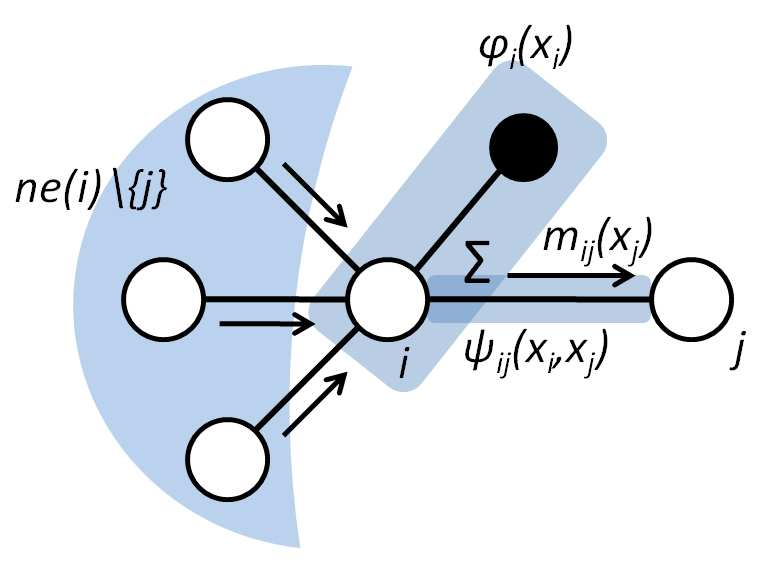
\includegraphics[scale=0.2]{schemaMRF.png}
  \end{figure}
\end{frame}

\begin{frame}
  \frametitle{Modélisation}
  \begin{itemize}
   \item Chaque phrase est modélisée par un noeud dans le graphe, qui est affecté de deux scores (contexte et non)
   \item Le nombre de dépendances est variable (c'est un paramètre testé).
   \item On note BPi le MRF où chaque noeud est lié à 2i voisins (i phrases précédentes, i phrases suivantes)
  \end{itemize}
\end{frame}

\begin{frame}
  \frametitle{Algorithme \textit{Belief Propagation}}
  \begin{itemize}
   \item Les scores de chaque noeud dépendent de ceux des noeuds voisins par \textit{message passing}
   \item Il y a convergence si les messages ne changent pas d'un certain seuil entre deux itérations
   \item En théorie la convergence n'est pas assurée pour les graphes mais en pratique BP converge toujours
  \end{itemize}
\end{frame}

\section{Experiences et résultats}
\begin{frame}
  \frametitle{Baselines}
  \begin{block}{Baseline "RI"}
  %\begin{itemize}
    Mesure de similarité entre les phrases contenant des citations
  %\end{itemize}
  \end{block}
  \begin{block}{Baseline "MRF"}
  %\begin{itemize}
    Cherche des motifs de discours dans le voisinnage des citations 
  %\end{itemize}
  \end{block}
\end{frame}

\begin{frame}
  \frametitle{Résultats}
  Résumé des résultats (F-mesure par article)
  \begin{itemize}
   \item Les scores sont très hétérogènes
   \item Le MRF version BP4 présente les meilleurs résultats
   \item Amélioration notable par rapport aux baselines
   \item Toutes méthodes confondues, moyenne à 0.3, max à 0.8
  \end{itemize}


\end{frame}

\section{Conclusion}
\begin{frame}
  \frametitle{Conclusion}

  \begin{itemize}
    \item Amélioration nette de la détection de citations implicites
    \item Apport d'information sur le contexte pour la génération de résumés
  \end{itemize}
\end{frame}

\section{Remarques}
\begin{frame}
  \frametitle{Remarques}

  \begin{itemize}
    \item Corpus choisi ?
    \item Apprentissage ? (SVM...)
    \item Baselines choisies ?
  \end{itemize}
  
  Vos remarques ou questions ?
\end{frame}

\end{document}
